\documentclass[11pt]{article}
\usepackage{style} 
\usepackage{placeins}
\usepackage{float}
\usepackage{setspace}
\usepackage{wrapfig}   % Assicurati che sia nel preamble


%================
% Title and Author Information
%================

\title{{\titlefont \textbf{Vertical Profiling of Atmospheric Parameters and Spectral Analysis during a CanSat Descent
}}}

\author{Alice Ferrini, Mattia De Martino}
\date{\today}

\usepackage{tcolorbox}

\begin{document}
\maketitle

\begin{center}
    \small\href{https://colab.research.google.com/github/mattiademartino/Space_Data_2/blob/main/main.ipynb}{\texttt{Google Colab Code}}
\end{center}



%================
% Document Start
%================
\setlength{\belowdisplayskip}{3pt} \setlength{\belowdisplayshortskip}{3pt}
\setlength{\abovedisplayskip}{3pt} \setlength{\abovedisplayshortskip}{0pt}

\section{Introduction}
\subsection{Mission Overview and Research Question}
On 5 February 2026, five CanSat probes were released from a light aircraft over Dübendorf, Switzerland, at approximately 600 m above ground level, as part of an analogue Venus mission. One probe was not launched due to a battery failure, and a second underwent an uncontrolled descent after its parachute failed to open, leaving four usable science datasets. As the probes descend freely under a parachute, their sensors are subject to oscillations and rotations that introduce periodic artefacts into the raw measurements. Spectral analysis is therefore the key tool to separate atmospheric variability from these mechanical disturbances, and forms the basis of our research question:

\begin{tcolorbox}[
    colback=gray!10,
    colframe=gray!50,
    boxrule=0.8pt,
    arc=4pt,
    left=8pt, right=8pt, top=6pt, bottom=6pt
]
\textit{How do temperature, pressure, particulate matter, CO\textsubscript{2}, and wind vary with altitude and time during the CanSat descent, and how can spectral analysis help distinguish atmospheric structure from sensor noise and oscillatory descent dynamics?}
\end{tcolorbox}

% Requires in preamble: \usepackage{tcolorbox}

\subsection{Data Quality Assessment}
A preliminary inspection of the four datasets evaluated their suitability for spectral analysis; the key parameters are summarised in Table~\ref{tab:cansat_summary}.

\textbf{OBAMA} transmitted only aggregated LoRa averages, providing insufficient temporal resolution for spectral analysis and is therefore excluded.

\textbf{GRASP} suffered a false trigger that caused recording to begin before the actual drop, introducing an abrupt discontinuity in the pressure and temperature profiles. GRASP is therefore also excluded.

\textbf{VAMOS} shows a clean, monotonically decreasing pressure profile during descent and physically plausible temperature readings throughout. Its additional CO\textsubscript{2} and wind measurements, together with an onboard tumbling flag, make it the richest dataset and it is selected as a primary dataset.

\textbf{ScamSat} covers the full flight from pre-launch to landing. The descent lasted 168,s over 665,m, with clean pressure and temperature profiles and no systematic artefacts. With additional PM\textsubscript{2.5}, PM\textsubscript{10}, acceleration, and audio channels, it is selected as the second primary dataset.

\begin{table}[ht]
\centering
\footnotesize
\setlength{\tabcolsep}{6pt}
\caption{Summary of the four CanSat science datasets and their suitability for spectral analysis.}
\label{tab:cansat_summary}
\begin{tabular}{lcccc}
\toprule
& \textbf{\textcolor{probeRed}{OBAMA}} & \textbf{\textcolor{probeRed}{GRASP}} & \textbf{\textcolor{probeGreen}{VAMOS}} & \textbf{\textcolor{probeGreen}{ScamSat}} \\
\midrule
$f_s$              & 0.02 Hz       & 38 Hz         & 1 Hz              & 1 Hz          \\
$N$ samples        & 23            & 1716          & $\approx$3550     & 9249          \\
Duration           & 6 min         & 3 min         & 99 min            & 59 min        \\
Pressure           & 900--946 hPa  & 812--874 hPa  & 868--950 hPa      & 870--940 hPa  \\
Temperature        & anomalous     & 14.5--24.1\,\textdegree C & 10.9--23.3\,\textdegree C & 10--22\,\textdegree C \\
Sensors            & Humidity      & PM$_{2.5}$, PM$_{10}$, Alt. & CO$_2$, Wind & PM$_{2.5}$, PM$_{10}$, Audio \\
\midrule
Role               & \textcolor{probeRed}{Excluded}   & \textcolor{probeRed}{Excluded}   & \textcolor{probeGreen}{Primary}  & \textcolor{probeGreen}{Primary}  \\
Reason             & Low $f_s$     & False trigger & Clean drop        & Clean drop    \\
\bottomrule
\end{tabular}
\end{table}


\subsection{Methods Overview}
To address the research question, spectral analysis is applied to the raw sensor time series recorded by VAMOS and ScamSat. By transforming the signals into the frequency domain, it is possible to identify characteristic frequencies associated with probe dynamics and distinguish them from the low-frequency atmospheric variability of interest. Once these mechanical disturbances are localised in frequency, the signal can be filtered to recover a clean atmospheric profile. The resulting data are then compared against external meteorological datasets to validate the physical consistency of the recovered signal and draw conclusions about the vertical structure of the atmosphere during the descent.


\subsection{Expected Results}

\noindent  \textbf{Probe dynamics.} In the time-frequency domain, we expect to identify stable, narrowband spectral peaks associated with pendulum oscillations (typically 0.1–0.5,Hz for parachute suspension lines of a few metres) and axial rotation. In the spectrogram, these should appear as continuous horizontal bands, persistent throughout the descent and clearly distinguishable from genuine atmospheric signals, which are expected to be broadband or slowly varying in frequency.

\noindent \textbf{Atmospheric conditions.} On 5 February 2026, Zürich was covered by a dense low-level radiation fog in the morning, which dissolved during the day, a signature of a pronounced temperature inversion and a particularly stable atmosphere \citep{meteoswiss_opendata}. Under such conditions, vertical motion and mixing is strongly suppressed, leading to temperature increasing with altitude within the inversion layer, weak wind speeds, and elevated CO\textsubscript{2} and particulate matter near the surface \citep{lohmann2024}. These expected signatures allow us to approach the data with a more critical eye when evaluating the results of the spectral analysis. 


\section{Methodology: Data Set and Analysis Workflow}
\subsection{Spectral Analysis}

\subsubsection{Purpose and signal preparation}
The aim of the spectral analysis is to identify disturbances that are not atmospheric in origin, such as parachute oscillations, payload rotations, and high-frequency sensor noise. Since the sensors are mounted on small probes descending under parachutes, part of the measured variability can be produced by the motion of the CanSat itself rather than by changes in temperature, pressure, particulate matter, CO\textsubscript{2}, or wind. The spectral workflow is therefore used as a diagnostic step before the atmospheric interpretation: it allows us to locate suspicious periodic components, remove them when justified, and retain a signal that is more representative of the real vertical structure of the atmosphere.

The workflow is applied to the usable high-quality datasets selected in the data quality assessment, with particular focus on VAMOS and ScamSat. For each variable, the relevant time interval is first isolated, invalid warm-up values are removed, and the samples are placed on a uniform time grid. This is necessary because FFT-based methods assume a constant sampling interval; otherwise, irregular timestamps would be incorrectly interpreted as changes in frequency content.

\subsubsection{Low-pass filtering}
A low-pass filter is first applied to reduce high-frequency sensor noise. The physical atmospheric signal is expected to vary slowly compared with the mechanical motion of the payload: pressure changes mainly because the probe descends, while temperature, CO\textsubscript{2}, and particulate matter evolve over comparatively long time scales. For this reason, a zero-phase Butterworth low-pass filter is used to smooth the raw profiles without shifting features in time or altitude. The cut-off frequency is chosen below the Nyquist frequency of each dataset and high enough to preserve the broad atmospheric trend.

\subsubsection{Trend removal}
After filtering, the dominant trend is removed when the goal is to study the residual signal in the frequency domain. This step is especially important for pressure and temperature, because the descent produces a large low-frequency component that can hide weaker periodic disturbances. A linear or low-order trend is subtracted from the uniformly sampled signal, and the remaining residual is treated as the approximately stationary time series used for spectral analysis. The residual is not interpreted as the final atmospheric profile; it is used only to detect periodic artefacts and sensor noise.

\subsubsection{FFT and Welch spectral estimation}
The detrended residuals are analysed with two complementary methods. A Hann-windowed FFT is used to inspect the amplitude of individual frequency components, while Welch's power spectral density (PSD) is used to estimate how the signal energy is distributed across frequency in a more stable way. Welch's method divides the signal into shorter overlapping windows, computes the spectrum of each window, and averages the result; this reduces the sensitivity to isolated transients and makes recurring oscillations easier to identify.

\begin{figure}[htbp]
    \centering
    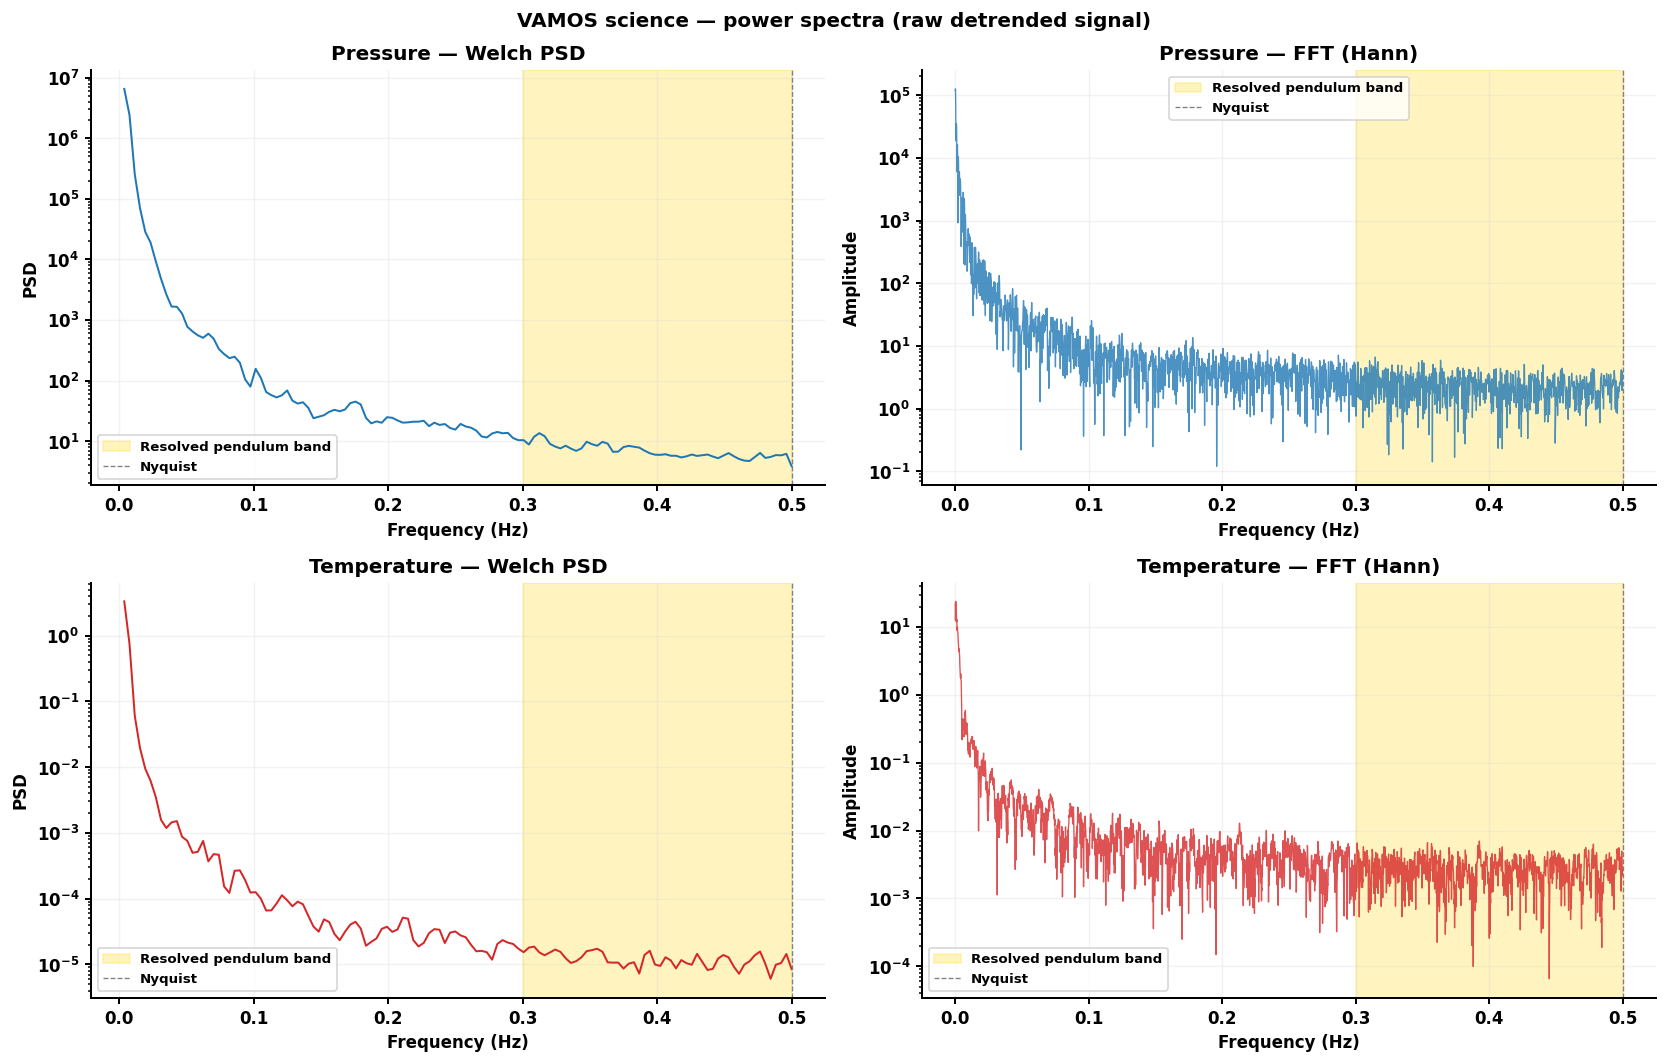
\includegraphics[width=0.92\linewidth]{Img/fig_vamos_psd.png}
    \caption{Example of the spectral diagnostic applied to VAMOS pressure and temperature. The raw signals are detrended before the Hann-windowed FFT and Welch PSD are computed. Because VAMOS is sampled at 1 Hz, the Nyquist frequency is 0.5 Hz; only the lower part of the expected pendulum range can be resolved, while faster spin modes would be aliased.}
    \label{fig:vamos_psd}
\end{figure}

Figure~\ref{fig:vamos_psd} shows the diagnostic logic used in the report. The expected parachute oscillation range is approximately 0.1--0.5 Hz for suspension lines of a few metres, but the 1 Hz sampling rate of VAMOS limits the resolvable spectrum to frequencies below 0.5 Hz. For this reason, only the lower part of the pendulum band can be evaluated, while faster axial rotations would be aliased and cannot be interpreted directly from these channels.

\subsubsection{Identification and removal of external disturbances}
The final step is to decide whether a frequency component can be attributed to an external disturbance. A component is considered suspicious only if it is narrowband, physically plausible, and persistent across the relevant diagnostics or flight phases. In the time-frequency domain, such a disturbance should appear as a stable horizontal band in the spectrogram, whereas atmospheric variability is expected to be slower, broader, or more transient.

If a clear mechanical frequency is found, the affected band is attenuated before reconstructing the cleaned signal. If no stable peak is present, no notch filter is imposed: in that case the atmospheric profiles are taken from the low-pass-filtered signal, avoiding the removal of physically meaningful variability. This conservative criterion is important because the goal is not simply to make the signal smoother, but to separate atmospheric structure from artefacts introduced by the CanSat descent dynamics.


\subsection{Data Analysis and Visualization}
\noindent Once the cleaned atmospheric signals are obtained, the processed variables are visualised to extract physically meaningful information about the vertical structure of the atmosphere during the descent. Temperature, pressure, CO\textsubscript{2}, and particulate matter (PM\textsubscript{2.5} and PM\textsubscript{10}) are plotted as vertical profiles, allowing direct inspection of how each quantity varies with altitude and enabling comparison with the expected signatures of the temperature inversion described above. Wind speed and direction are visualised using a compass rose, showing the distribution of wind directions and their associated magnitudes, and a hodograph, a graph in which the east--west and north--south components of the wind vector are plotted against each other at successive altitude levels \citep{lohmann2024}. This representation reveals how wind speed and direction evolve with height, providing insight into the vertical wind shear structure of the boundary layer during the descent. 


\subsection{External Datasets Comparison}
To validate the cleaned atmospheric profiles, \textbf{five} external datasets are used as reference. Since each carries its own limitations, they are used in combination, selecting the most appropriate one depending on the variable under analysis.

\subsubsection{International Standard Atmosphere (ISA)}
\subsubsection{Payerne Radiosonde}
\subsubsection{ERA5 Reanalysis}
\subsubsection{MeteoSwiss Ground Stations: Zürich/Fluntern and Üetliberg}
\subsubsection{E-PROFILE EUMETNET: Celiometer}



\section{Results}
\input{Text/Results} 

\titlespacing*{\section}{0pt}{*2}{*1}
\section{Interpretation and Discussion}
\input{Text/Interpretation and Discussion} 

\setlength{\belowdisplayskip}{0pt} \setlength{\belowdisplayshortskip}{0pt}
\setlength{\abovedisplayskip}{0pt} \setlength{\abovedisplayshortskip}{0pt}

\small
\setstretch{1}
\setlength{\bibsep}{0pt plus 0.3ex}
\bibliographystyle{unsrtnat}
\titlespacing*{\section}{0pt}{*1}{*0.5}
% \bibliographystyle{unsrt}
{\footnotesize\bibliography{references.bib}}



\end{document}